\section{Overview}
\label{sec:ktoctou-overview}




\subsection{Threat Model}
\label{sec:ktoctou-threatmodel}

Kernel TOCTOU is a local privilege escalation vulnerability. The vulnerability could allow local users or malicious software to gain full root privileges. We assume an attacker has a user account that can upload and run arbitrary programs with user privilege, or he can access such a program. The attacker has arbitrary memory read and writes primitives. He is also able to call any system services or load any library. The DEP policy (\textbf{W}rite $\oplus$ e\textbf{X}ecute) and ASLR is not necessary. We assume the attacker has full knowledge about the system kernel, including the memory layout. However, he can not read or write any kernel memory as a classical operating system would not allow. The attacker aims at running arbitrary code in the kernel, hence obtain the highest privilege. 

We aim at the Windows OS, a complicated operating system. \name will not work on the Linux kernel because it already utilizes the Intel CPU feature SMAP in a conventional way. We will elaborate on this in~\autoref{sec:ktoctou-background}.

%Without investigation,  we can not be sure that the mitigation will work on other OS, even the underlying mechanism should work.\hb{you dont need to write this in the threat model} 

Considering we leverage a hardware feature from Intel CPU, The host system should use Intel CPU with SMAP capability.


\subsection{High-Level Design and Challenges}

The kernel double fetching a user address may cause a TOCTOU vulnerability. From a practical point of view, we can not make the kernel change its double-fetch behavior. Instead, we want to make the two fetches always get the same value, thus no vulnerability. The high-level idea is as follows.  When the kernel accesses a user address, we froze the containing page so that no other user thread can overwrite it.


The main challenges are:

\begin{itemize}
	\item How can we know when the kernel accesses a user address?
	\item It is overkill to froze an entire page just for one variable, and reads should allow.
	\item The two fetches should happen within a short time, more specifically, within the same system call. 
	\item Windows is a complex operating system, if not the most complex system. How is it practical to enable a system-wide hardware feature such as SMAP without crash the system?
\end{itemize}


\subsection{Approach Overview}


When the kernel accesses a user address, how to get notified is the most challenging issue. Because the processor reading memory is such an ordinary operation, no official hardware feature is available for monitoring that in a broad range of memory. We abuse a hardware feature SMAP. It was initially designed to prevent the attacker from tricking the kernel into getting shellcode or malicious data from userspace. However, one main character of this feature is that when the kernel accesses a user address, the processor raises a page fault exception. This part accurately serves our purpose, so we want to leverage it in a novel way.

Subject to the x86 architecture, the protection has to base on a page granularity. To protect even one byte, we have to deal with an entire page.
First, we separate the subsequent user reads from writes. The reads are harmless.  When we temporarily release a page, we also set this page as read-only to ensure no writing. When a user writes on the protected page, we make the thread suspend on the writing instruction and wait until the current system call ends.

As previously mentioned in ~\autoref{sec:ktoctou-background}, the kernel-level TOCTOU problems happen inside individual system calls. We hook Windows internal functions to known when a system call ends and release the pages the system call accessed. Also, we monitor the creation and termination for both processes and threads and use Windows internal data structures to distinguish each thread, namely, TEB.

We develop a light-weight hypervisor to confine the SMAP feature into specific processes. It makes debugging less painful to us, and it is also necessary to prevent nested SMAP exceptions that cause a dead loop.

~\autoref{fig:ktoctou-overview} shows the high-level overview. The hypervisor enables SMAP in one process, that is, the current one in the figure. The kernel accessed three user pages, as marked in the user process memory space. One user thread in the same process tries to access those pages. The read is allowed, where the page is released and set read-only. However, the write is not allowed for the moment; the page fault handler suspends the write to avoid any data inconsistency in the kernel.


\begin{figure}[th]
  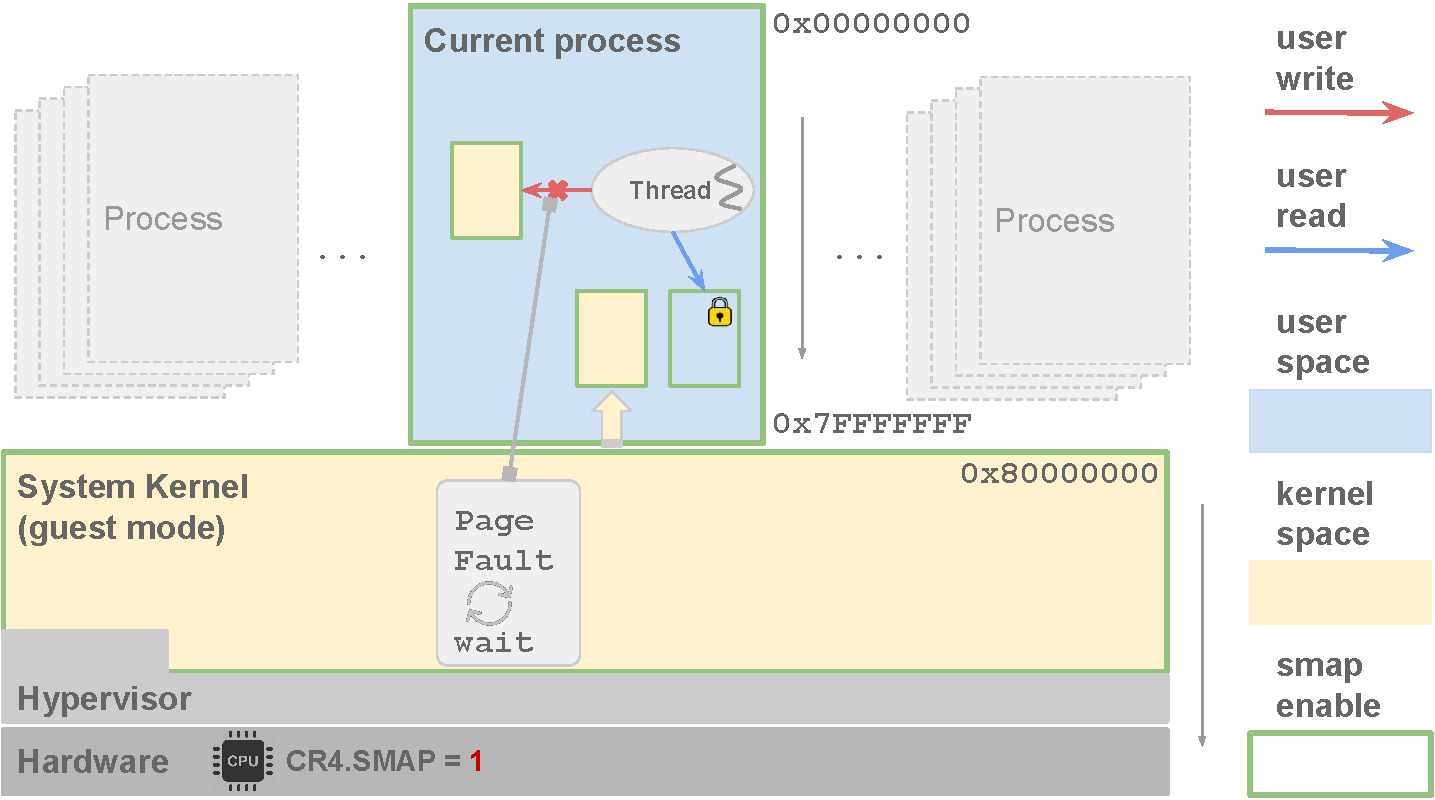
\includegraphics[width=0.47\textwidth]{figures/ktoctou-overview}
  \centering
  \caption{The hypervisor is capable of confining the system-wide feature SMAP into one process. The processor raises page fault exception when the kernel accesses userspace so that we can protect those pages. Other user threads can read a protected page but can not write. The write will raise another page fault exception, where the page fault handler will block the write instruction until the system call ends.}
  \label{fig:ktoctou-overview}
\end{figure}
